\subsection{Misure e osservazioni preliminari}

\subsubsection{Punto di lavoro del PMT2}

Vogliamo trovare un buon punto di lavoro per il PMT2 che è alimentato con tensioni positive fino a $\sim \SI{800}{V}$. 
Mandiamo il segnale preamplificato del PMT2 all'amplificatore e la sua uscita all'ADC in modalità automatica.
Scegliamo di alimentare il PMT2 alla tensione consigliata di \SI{650}V. A questa tensione (e con guadagno dell'amplificatore impostato a $\times 1$) il fotopicco generato dai fotoni più energetici tra le sorgenti a disposizione (ovvero il picco a \SI{1.33}{MeV} del \co) si trova a $2/3$ della scala. Questo permette, agendo sul fattore di amplificazione del formatore/amplificatore di portare il fotopicco a fondo scala  e massimizzare la risoluzione dello spettrometro, mantenendo allo stesso tempo flessibilità nel caso la risposta del rivelatore non si rivelasse stabile\footnote{Cosa che abbiamo verificato essere vera: la posizione dei fotopicchi può variare nel tempo fino al $\sim 10\%$.}.

\subsubsection{Stabilità della risposta del PMT2}

Notiamo che la risposta dello spettrometro è molto sensibile alle variazioni della tensione di alimentazione:
variando da \SI{600}V a \SI{575}V, la posizione dei fotopicchi si dimezza.
Il manuale dell'alimentatore riporta una stabilità dello \SI{0.5}{\permil} su \SI{24}h e dell'\SI1{\permil} su un mese. Volendo fare una stima otteniamo variazioni del $2/25 \times 600/1000 = \SI5\%$ in un mese, la metà in \SI{24}h. Sembra quindi che la stabilità della risposta del nostro spettrometro sia un limite importante nella nostra misura per cui nel seguito analizzeremo approfonditamente questo parametro.
%%%%%%%%%%%%%%%%%%%%%%%%%%%%%%%%%%%%%%%%%%%%%%%%%%%%%%%%%%%

\subsubsection{Interazione con il bersaglio}

Poniamo lo scintillatore plastico (PMT1) davanti alla sorgente in modo che i raggi~$\gamma$ possano interagire e subire scattering Compton. Osserviamo l'istogramma dei campionamenti del nostro spettrometro a vari angoli rispetto al bersaglio (ne riportiamo due in \autoref{4ang}) mentre l'ADC campiona in modalità automatica.
Il range dei fotoni del \co\; nel bersaglio è $\sim\SI{10}{cm}$ e il suo spessore $\sim\SI{1}{cm}$, quindi solo il $10\%$ dei fotoni interagisce. 
Se lo spettrometro si trova a piccolo angolo rispetto al bersaglio viene attraversato dai fotoni che non hanno interagito e lo spettro è sostanzialmente uguale a quello acquisito senza bersaglio. A grande angolo vorremmo vedere i fotoni che fanno Compton sul bersaglio e arrivano con un certo angolo di scattering sul rivelatore (producendo quindi uno spettro simile al precedente ma traslato a energie minori) ma i fotoni che non interagiscono proseguono sino al muro subito dietro lo spettrometro, una parte di questi fa scattering Compton o Rayleigh e può arrivare nello spettrometro, sovrastando in statistica il segnale che vorremmo osservare.

\begin{figure}[h]
	\centering
	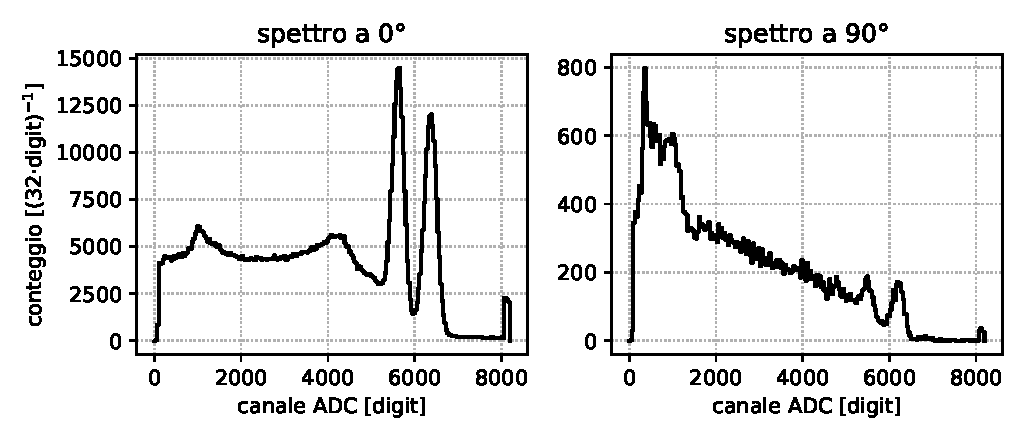
\includegraphics[width=\textwidth]{plotg}
	\caption{Spettri raccolti senza coincidenza a diversi angoli rispetto al bersaglio.}
	\label{4ang}
\end{figure}

Abbiamo poi confrontato lo spettro a \SI{45}{\degree} con o senza scintillatore plastico, ma non abbiamo notato nessuna differenza. Abbiamo anche verificato che, come atteso, il rate di eventi diminuisce all'aumentare della distanza.

Proviamo a schermare lateralmente lo scintillatore cristallino con il piombo per ridurre il fondo di backscattering e lo spettro in \autoref{casetta} mostra come effettivamente questo si riduca ma non a sufficienza da poter osservare il segnale.
\marginpar{Dalla \autoref{casetta} non mi sembra che il backscattering si riduca,
ma piuttosto che compaia un picco a sinistra.\\
\emph{Petrillo}}
Si rende necessario l'uso di un trigger esterno per campionare sulla coincidenza di segnale tra PMT1 e PMT2.

\begin{figure}
	\centering
	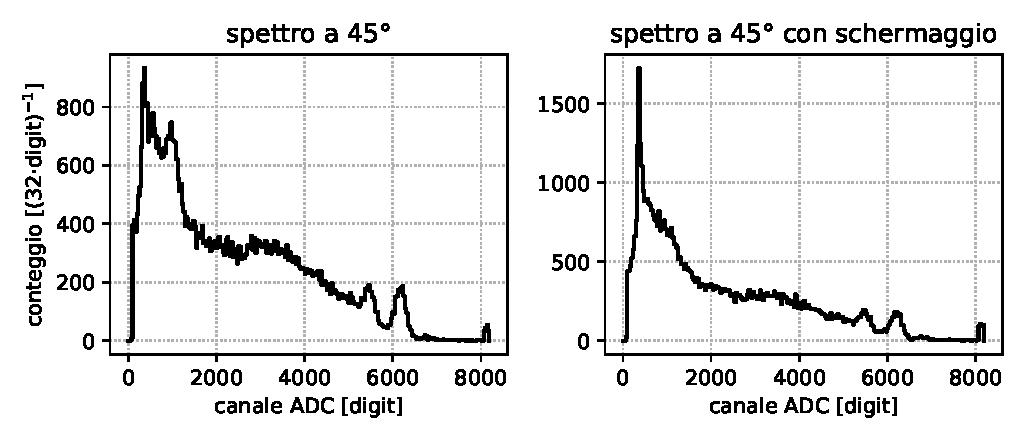
\includegraphics[width=\textwidth]{plotcasetta}
	\caption{Confronto tra gli spettri a 45$^{\circ}$ con e senza schermaggio.}
	\label{casetta}
\end{figure}

\subsubsection{Trigger esterno}
Per ottenere il segnale di trigger usiamo il circuito in \autoref{fig:trigger}:\marginpar{aggiungere figura?(Bob)}
\begin{itemize}
	\item il segnale ``veloce'' del PMT2 (quello non pre-amplificato con ampiezza di picco $\sim\SI{20}{mV}$) è prima amplificata di un fattore 10 attraverso un modulo di amplificazione lineare, quindi inviato ad un discriminatore con soglia a $\SI{35}{mV}$ (il minimo) in modo da ottenere una soglia efficace più bassa;
	\item il segnale del PMT1 è inviato direttamente ad un discriminatore con soglia a $\SI{35}{mV}$ (il minimo);
	\item entrambi gli output dei discriminatori vanno ad un sistema di anti-retrigger che impone un tempo morto di $\sim\SI{1}{\micro s}$ e produce segnali di durata $\sim\SI{30}{ns}$;
	\item il segnale discriminato del PMT1 è ritardato di circa \SI{20}{ns} per compensare un ritardo asimmetrico dovuto al modulo di anti-retrigger;
	\item facciamo la coincidenza dei due segnali così formati e mandiamo l'output a un modulo \texttt{gate \& delay}.
	\item l'ADC richiede un segnale di trigger che parta almeno \SI{200}{ns} prima del picco e termini almeno \SI{200}{ns} dopo: usando l'oscilloscopio, regoliamo il modulo \texttt{gate \& delay} in modo da avere un segnale della durata di $\sim\SI{1}{\micro s}$ centrato sul picco del formatore.
\end{itemize}
Acquisiamo degli spettri di prova e verifichiamo che con le soglie impostate i primi $\sim1000$ canali dell'ADC non mostrano campionamenti.

\subsubsection{Punto di lavoro del PMT1}
Il PMT1 può essere alimentato fino a \SI{1800}{V} e nel range \SI{1500}{V}-\SI{1700}{V} mostra circa lo stesso rate. Decidiamo di alimentarlo a \SI{1700}{V} per avere alta efficienza e mantenendo il rate ragionevole.
\marginpar{tenerlo lontano da 1800\! V non conta niente? \\ (Andrea)}

\subsubsection{Stabilità della risposta del PMT2}

\begin{figure}
	\centering
	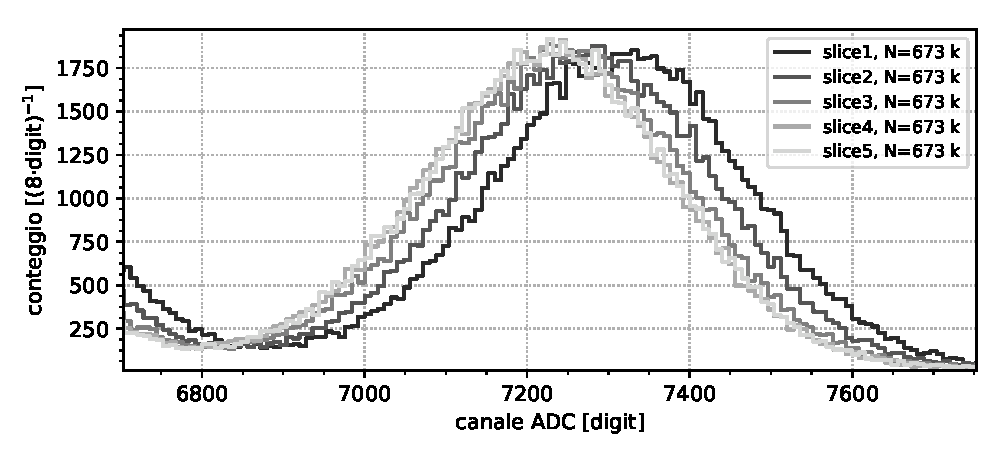
\includegraphics[width=\textwidth]{stability}
	\caption{\label{fig:stability}
	Dettaglio dello spettro del \co{}
	ottenuto da un'acquisizione di 25 ore
	separata in 5 parti da 5 ore.
	Si nota uno spostamento verso sinistra.}
\end{figure}

Una sorgente di errore sistematico che ci aspettiamo importante\footnote{Come vedremo sarà la principale componente dell'errore sulla misura finale.} è dovuta alla stabilità della risposta del nostro spettrometro. Per avere un idea della stabilità nel tempo della calibrazione campioniamo per $\sim\SI{25}{h}$ lo spettro del \co, quindi dividiamo i dati in parti di uguale statistica (che a rate costante implicano circa durate uguali) e grafichiamo. In \autoref{fig:stability} è riportato il risultato per intervalli temporali di $\sim\SI{5}{h}$: la calibrazione varia in $\SI{24}{h}$ di poco più del \SI2\% e la variazione non è costante nel tempo, ma concentrata soprattutto nelle prime ore.

Stimiamo qual è l'effetto dell'instabilità.
Invertendo la \eqref{energia_compton} otteniamo
\begin{equation}
	\label{eq:scalibur}
	\left. \pdv{m_e}{E'} \right|_\theta = \frac{1-\cos\theta}{\left( 1-\frac{E'}{E}\right )^2}
\end{equation}
che, poiché $E$ e $\theta$ sono conosciuti con precisione e misuriamo $E'$ con lo spettrometro,
ci dà come varia la massa dell'elettrone misurata dal nostro esperimento quando l'apparato si scalibra.
Ad esempio per $E=\SI{1.33}{MeV}$ e $\theta=\SI{10}{\degree}$ abbiamo $E'\approx\SI{1.28}{MeV}$ e,
ammettendo una variazione della calibrazione del \SI1\%
(dato realistico alla luce delle misure precedenti),
otteniamo una variazione della massa misurata
\begin{align*}
	\Delta m_e
	\approx \frac{1-\cos\theta}{\left( 1-\frac{E'}{E}\right )^2} \cdot \frac{\Delta E'}{E'} \cdot E'
	\approx \frac{0.015}{0.0014} \cdot \SI1\% \cdot \SI{1.28}{MeV}
	= \SI{0.14}{MeV}.
\end{align*}
Questo ci mostra come le misure dell’elettrone a piccolo angolo saranno dominate da questo errore.
